%%%%%%%%%%%%%%%%%%%%%%%%%%%%%%%%%%%%%%%%%%%
%
% From a template maintained at https://github.com/jamesrobertlloyd/cbl-tikz-poster
%
% Code near the top should be fairly standard and not need to be changed
%  - except for the document class
% Code lower down is more likely to be customised
%
%%%%%%%%%%%%%%%%%%%%%%%%%%%%%%%%%%%%%%%%%%%

%%%%%%%%%%%%%%%%%%%%%%%%%%%%%%%%%%%%%%%%%%%
%
% Document class
%
% Change this if you want a different size / orientation poster etc
%
%%%%%%%%%%%%%%%%%%%%%%%%%%%%%%%%%%%%%%%%%%%

\documentclass[landscape,a0b,final,a4resizeable]{a0poster}
%\documentclass[portrait,a0b,final,a4resizeable]{a0poster}


\usepackage{multicol}
\usepackage{color}
\usepackage{shadow}
\usepackage{morefloats}
\usepackage{cite}
\usepackage[pdftex]{graphicx}
\usepackage{rotating}
\usepackage{amsmath, amsthm, amssymb, bm}
\usepackage{array}
\usepackage{nth}
\usepackage[square,numbers]{natbib}
\usepackage{booktabs}
%\usepackage{xcolor}

%%%%%%%%%%%%%%%%%%%%%%%%%%%%%%%%%%%%%%%%%%%
%
% TIKZ packages and common definitions
%
% Add extra things as per your tikz needs
%
%%%%%%%%%%%%%%%%%%%%%%%%%%%%%%%%%%%%%%%%%%%

\usepackage{../common/picins}
\usepackage{tikz}
\usetikzlibrary{shapes.geometric,arrows,chains,matrix,positioning,scopes,calc}
\tikzstyle{mybox} = [draw=white, rectangle]

%%%%%%%%%%%%%%%%%%%%%%%%%%%%%%%%%%%%%%%%%%%
%
% myfig
%
% \myfig - replacement for \figure
% necessary, since in multicol-environment 
% \figure won't work        
%                 
%%%%%%%%%%%%%%%%%%%%%%%%%%%%%%%%%%%%%%%%%%%

\newcommand{\myfig}[3][0]{
\begin{center}
  \vspace{1.5cm}
  \includegraphics[width=#3\hsize,angle=#1]{#2}
  \nobreak\medskip
\end{center}}

%%%%%%%%%%%%%%%%%%%%%%%%%%%%%%%%%%%%%%%%%%%
%
% mycaption                
%
% \mycaption - replacement for \caption
% necessary, since in multicol-environment \figure and
% therefore \caption won't work
%
%%%%%%%%%%%%%%%%%%%%%%%%%%%%%%%%%%%%%%%%%%%

%\newcounter{figure}
\setcounter{figure}{1}
\newcommand{\mycaption}[1]{
  \vspace{0.5cm}
  \begin{quote}
    {{\sc Figure} \arabic{figure}: #1}
  \end{quote}
  \vspace{1cm}
  \stepcounter{figure}
}

%%%%%%%%%%%%%%%%%%%%%%%%%%%%%%%%%%%%%%%%%%%
%
% Some standard colours
%
%%%%%%%%%%%%%%%%%%%%%%%%%%%%%%%%%%%%%%%%%%%

\definecolor{camlightblue}{rgb}{0.601 , 0.8, 1}
\definecolor{camdarkblue}{rgb}{0, 0.203, 0.402}
\definecolor{camred}{rgb}{1, 0.203, 0}
\definecolor{camyellow}{rgb}{1, 0.8, 0}
\definecolor{lightblue}{rgb}{0, 0, 0.80}
\definecolor{white}{rgb}{1, 1, 1}
\definecolor{whiteblue}{rgb}{0.80, 0.80, 1}

%%%%%%%%%%%%%%%%%%%%%%%%%%%%%%%%%%%%%%%%%%%
%
% Some look and feel definitions
%
%%%%%%%%%%%%%%%%%%%%%%%%%%%%%%%%%%%%%%%%%%%

\setlength{\columnsep}{0.03\textwidth}
\setlength{\columnseprule}{0.0018\textwidth}
\setlength{\parindent}{0.0cm}

%%%%%%%%%%%%%%%%%%%%%%%%%%%%%%%%%%%%%%%%%%%
%
% \mysection - replacement for \section*
% 
% Puts a pretty box around some text
% TODO - any other thoughts for what this box should look like
%
%%%%%%%%%%%%%%%%%%%%%%%%%%%%%%%%%%%%%%%%%%%

\tikzstyle{mysection} = [rectangle, 
									draw=none, 
									shade, 
									outer color=camlightblue!30,
									inner color=camlightblue!30,
									text width=0.965\columnwidth,
									text centered,
									rounded corners=20pt,
									minimum height=0.11\columnwidth]

\newcommand{\mysection}[1]
{
\begin{center}
  \begin{tikzpicture}
    \node[mysection] {\sffamily\bfseries\LARGE#1};
  \end{tikzpicture}
\end{center}
}

%%%%%%%%%%%%%%%%%%%%%%%%%%%%%%%%%%%%%%%%%%%
%
% Set the font
%
% TODO - Not sure what a canonical choice is - feel free to modify
%
%%%%%%%%%%%%%%%%%%%%%%%%%%%%%%%%%%%%%%%%%%%

\renewcommand{\familydefault}{cmss}
\sffamily

%%%%%%%%%%%%%%%%%%%%%%%%%%%%%%%%%%%%%%%%%%%
%
% Poster environment
%
% Centres everything and can be used to define the width of the content
%
%%%%%%%%%%%%%%%%%%%%%%%%%%%%%%%%%%%%%%%%%%%

\newenvironment{poster}{
  \begin{center}
  \begin{minipage}[c]{0.96\textwidth}
}{
  \end{minipage} 
  \end{center}
}

%%%%%%%%%%%%%%%%%%%%%%%%%%%%%%%%%%%%%%%%%%%
%
% This is probably a good place to put content specific packages and definitions
%
%%%%%%%%%%%%%%%%%%%%%%%%%%%%%%%%%%%%%%%%%%%

\usepackage{preamble}
\usepackage{tabularx}

\def\newarrow{\mbox{\begin{tikzpicture}
             \useasboundingbox{(-3pt,-4.5pt) rectangle (19pt,1pt)};
             \draw[->] (0,-0.07)--(17pt,-0.07);\end{tikzpicture}}}

%%%%%%%%%%%%%%%%%%%%%%%%%%%%%%%%%%%%%%%%%%%
%
% The document environment starts here
%
%%%%%%%%%%%%%%%%%%%%%%%%%%%%%%%%%%%%%%%%%%%

\begin{document}

%%%%%%%%%%%%%%%%%%%%%%%%%%%%%%%%%%%%%%%%%%%
%
% Begin the poster environment - centres things and potentially changes the width
%
%%%%%%%%%%%%%%%%%%%%%%%%%%%%%%%%%%%%%%%%%%%

\begin{poster}

%%%%%%%%%%%%%%%%%%%%%%%%%%%%%%%%%%%%%%%%%%%
%
% Potentially add some space at the top of the poster
%
%%%%%%%%%%%%%%%%%%%%%%%%%%%%%%%%%%%%%%%%%%%

\vspace{0\baselineskip}

%%%%%%%%%%%%%%%%%%%%%%%%%%%%%%%%%%%%%%%%%%%
%
% Draw the header as a TIKZ picture
%
% Using TIKZ to allow for easy alignment
%
%%%%%%%%%%%%%%%%%%%%%%%%%%%%%%%%%%%%%%%%%%%

\begin{center}
\begin{tikzpicture}[x=0.5\textwidth]
    % Dummy nodes at edges for spacing
    % TODO - a better way?
    \node at (+1, 0) {};    
    \node at (-1, 0) {};
    % Set the size of the badges
    \def \badgeheight {0.08\textwidth}
    % Title text
    \node[inner sep=0,text width=0.7\textwidth,text centered,font=\Huge] (Title) at (0,0) 
    {
      {\sffamily \Huge \textbf{Automatic construction and description of nonparametric models}}\\
      {\huge\sffamily James Robert Lloyd\textsuperscript{1}, {David Duvenaud}\textsuperscript{1}, Roger Grosse\textsuperscript{2},}\\
      \vspace{-0.1\baselineskip}
      {\huge\sffamily Joshua B. Tenenbaum\textsuperscript{2}, Zoubin Ghahramani\textsuperscript{1}}\\
      \vspace{-0.3\baselineskip}
      {\large\sffamily 1: Department of Engineering, University of Cambridge, UK 2: Massachusetts Institute of Technology, USA}
    };
    % Cambridge badge
    \node [mybox] (Cambridge Badge) at (-0.9, 0) {
        \includegraphics[height=\badgeheight]{../badges/cam-crest-and-text.pdf}
    };
    % CBL badge
    \node [mybox] (CBL Badge) at (-0.75, 0) {
        
\includegraphics[height=\badgeheight]{../badges/cbl-badge-cropped.png}
    };
    % MIT badge
    \node [mybox] (MIT Badge) at (+0.72, 0) {
        
\includegraphics[height=\badgeheight]{../badges/MIT2.jpg}
    };
     QR code
    \node [mybox] (QR code) at (+0.9, 0) {
        
\includegraphics[height=\badgeheight]{../badges/auto-stat-qr.png}
    };
\end{tikzpicture}
\end{center}

%%%%%%%%%%%%%%%%%%%%%%%%%%%%%%%%%%%%%%%%%%%
%
% Spacing between title and main body
%
%%%%%%%%%%%%%%%%%%%%%%%%%%%%%%%%%%%%%%%%%%%

\vspace{1\baselineskip}

%%%%%%%%%%%%%%%%%%%%%%%%%%%%%%%%%%%%%%%%%%%
%
% Columns environment
%
%%%%%%%%%%%%%%%%%%%%%%%%%%%%%%%%%%%%%%%%%%%

\begin{multicols}{3}

%%%%%%%%%%%%%%%%%%%%%%%%%%%%%%%%%%%%%%%%%%%
%
% Start of content
%
%%%%%%%%%%%%%%%%%%%%%%%%%%%%%%%%%%%%%%%%%%%

\large

\mysection{This analysis was automatically generated}

\vspace{0.5\baselineskip}

\begin{center}
\fbox{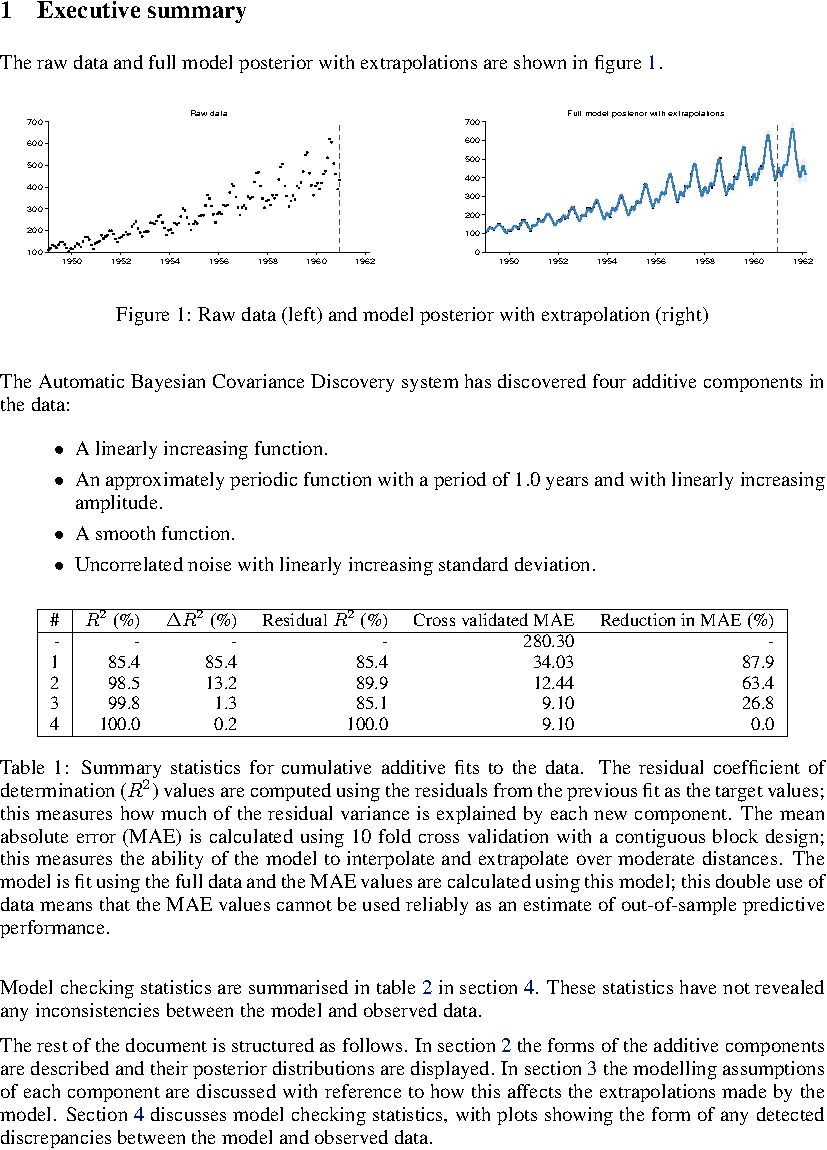
\includegraphics[trim=0cm 9.5cm 0cm 0.7cm, clip, width=0.98\columnwidth]{../figures/airline-pages/pg_0002-crop.pdf}}
%\fbox{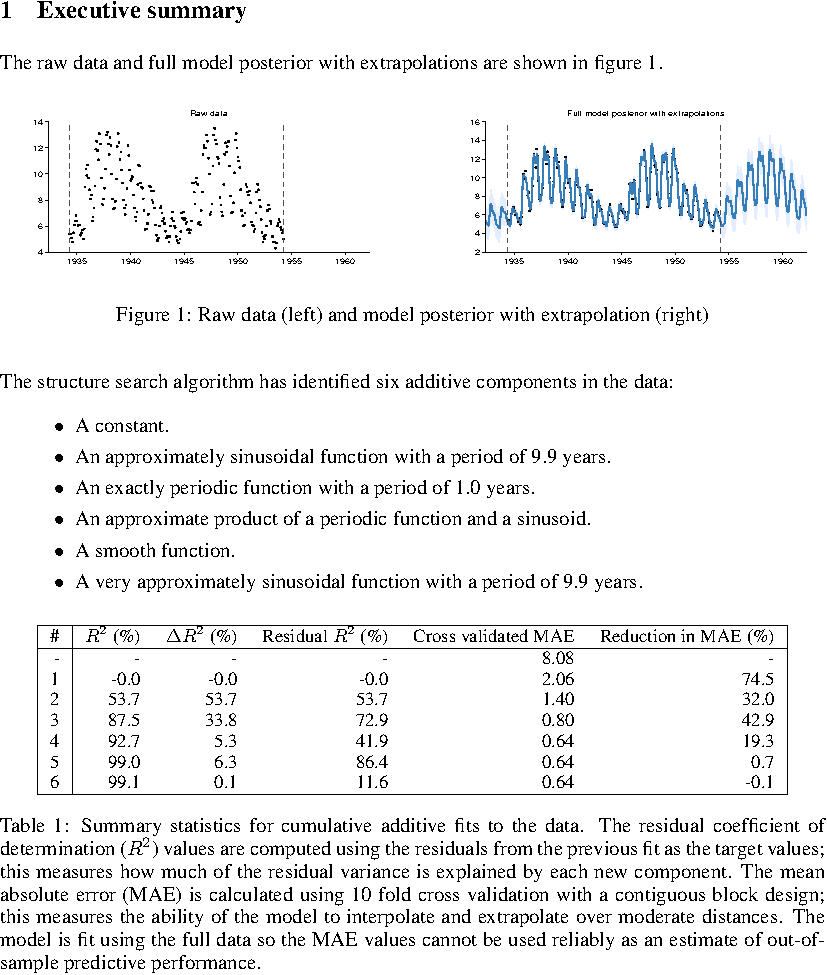
\includegraphics[trim=0cm 6.5cm 0cm 0.7cm, clip, width=0.98\columnwidth]{../figures/radio-pages/pg_0002-crop.pdf}}

\vspace{\baselineskip}
%\vspace{0.8\baselineskip}

\fbox{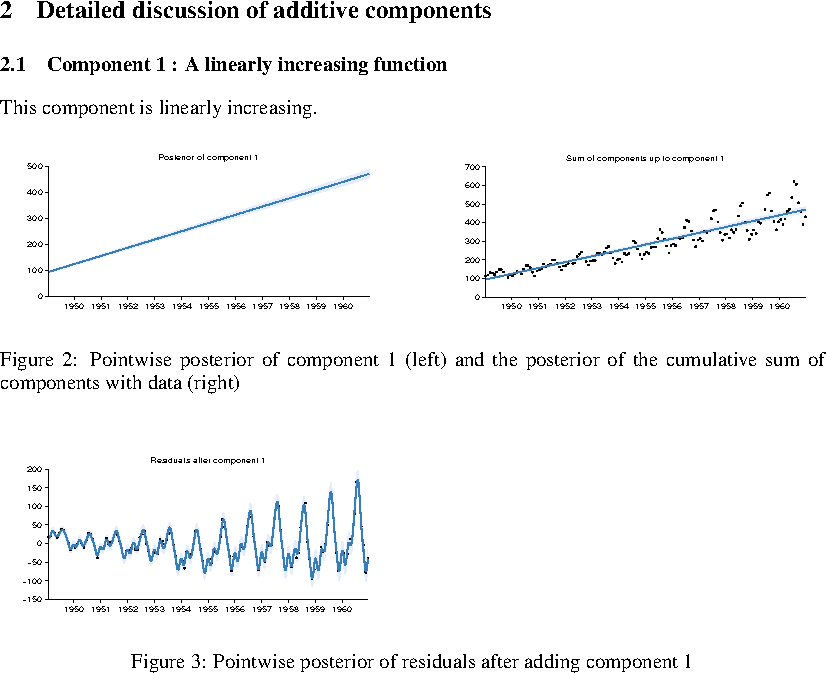
\includegraphics[trim=0cm 6cm 0cm 0.9cm, clip, width=0.98\columnwidth]{../figures/airline-pages/pg_0003-crop.pdf}}
%\fbox{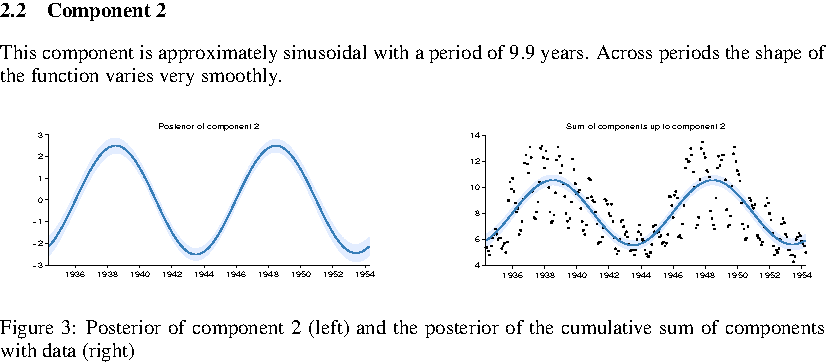
\includegraphics[trim=0cm 1cm 0cm 0.0cm, clip, width=0.98\columnwidth]{../figures/radio-pages/pg_0004-crop.pdf}}

\vspace{\baselineskip}
%\vspace{0.8\baselineskip}

\fbox{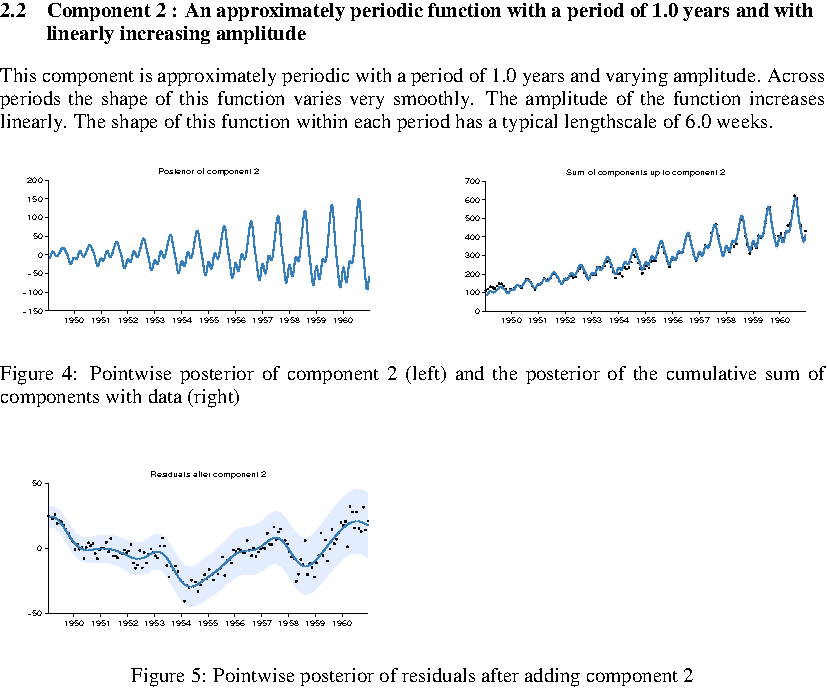
\includegraphics[trim=0cm 6cm 0cm 0.0cm, clip, width=0.98\columnwidth]{../figures/airline-pages/pg_0004-crop.pdf}}
%\fbox{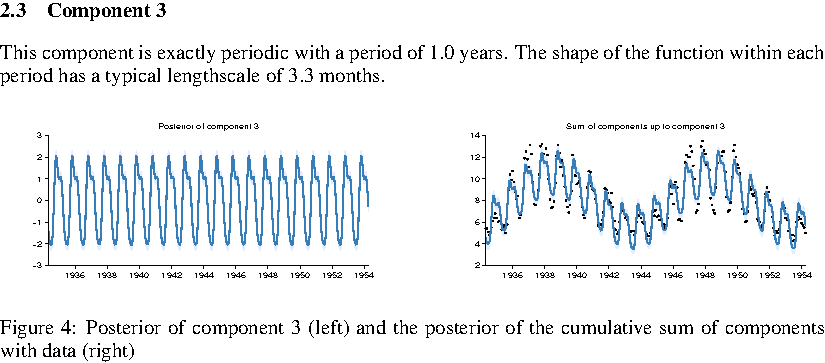
\includegraphics[trim=0cm 1cm 0cm 0.0cm, clip, width=0.98\columnwidth]{../figures/radio-pages/pg_0005-crop.pdf}}

\vspace{\baselineskip}
%\vspace{0.8\baselineskip}

\fbox{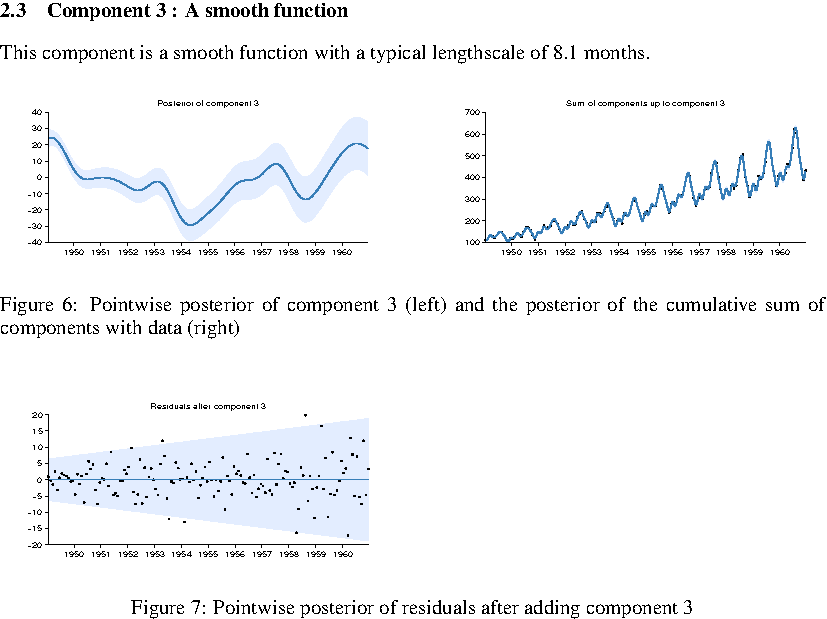
\includegraphics[trim=0cm 6cm 0cm 0.0cm, clip, width=0.98\columnwidth]{../figures/airline-pages/pg_0005-crop.pdf}}
%\fbox{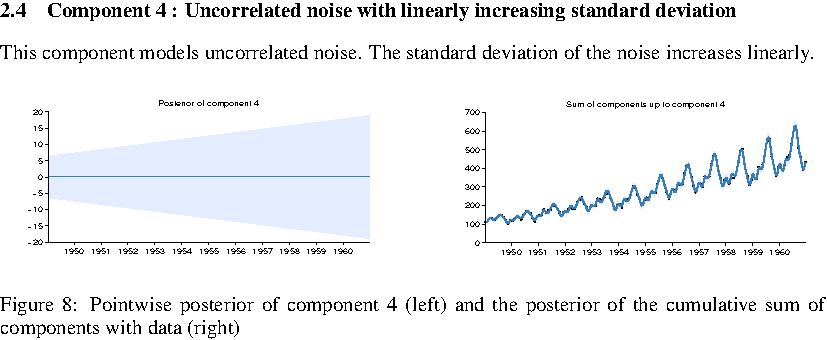
\includegraphics[trim=0cm 1cm 0cm 0.0cm, clip, width=0.98\columnwidth]{../figures/airline-pages/pg_0006-crop.pdf}}
%\fbox{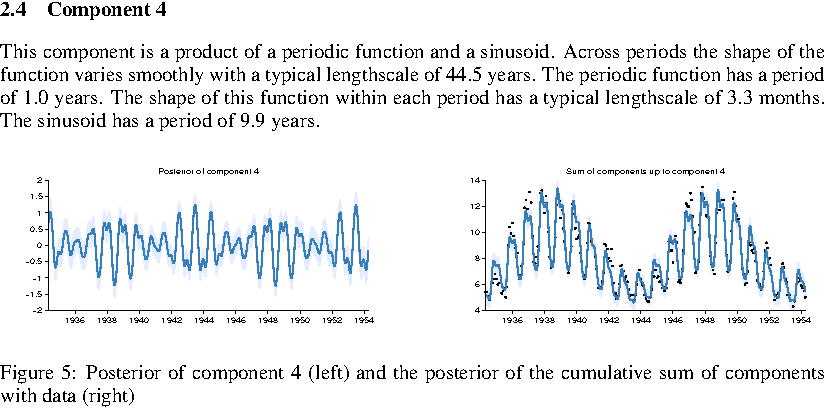
\includegraphics[trim=0cm 1cm 0cm 0.0cm, clip, width=0.98\columnwidth]{../figures/radio-pages/pg_0006-crop.pdf}}

\end{center}

\newpage 

\mysection{Modelling structure through\\Gaussian process kernels}

\vspace{0.5\baselineskip}

\begin{itemize}
  %\item The kernel determines which structures are likely under the \gp{} prior  
  %\item This prior determines the generalization properties of the model.
  %\item The kernel determines the pattern of generalization beyond the observed data
  \item The kernel specifies which structures are likely under the GP prior \\ - which determines the generalisation properties of the model.
  %For Gaussian process models, the prior --- and hence, the pattern of generalisation --- is determined by a kernel function. Common examples include:
  %\item Only a few simple kernels are commonly used \eg%the following standard kernels is used%\gp{} priors are used:
\end{itemize}
\vspace{1\baselineskip}
\newcommand{\fhbig}{5.0cm}
\newcommand{\fwbig}{5.625cm}
\newcommand{\kernpic}[1]{\includegraphics[height=\fhbig,width=\fwbig]{../figures/structure_examples/#1}}
\newcommand{\kernpicr}[1]{\rotatebox{90}{\includegraphics[height=\fwbig,width=\fhbig]{../figures/structure_examples/#1}}}
\newcommand{\addkernpic}[1]{{\includegraphics[height=\fhbig,width=\fwbig]{../figures/additive_multi_d/#1}}}
\newcommand{\largeplus}{\tabbox{{\Large+}}}
\newcommand{\largeeq}{\tabbox{{\Large=}}}
\newcommand{\largetimes}{\tabbox{{\Large$\times$}}}
\centering
\renewcommand{\tabularxcolumn}[1]{>{\arraybackslash}m{#1}}
%\begin{tabular}{m{\fwbig}m{0.01\textwidth}m{\fwbig}m{0.01\textwidth}m{\fwbig}m{\fwbig}m{\fwbig}}
%\begin{tabular}{C{\fwbig}C{\fwbig}C{\fwbig}C{\fwbig}}%{m{\fwbig}m{\fwbig}m{\fwbig}}
\begin{tabularx}{0.8\columnwidth}{XXXX}
%Composite & Draws from \gp{} & \gp{} posterior \\ \toprule
  \kernpic{se_kernel_draws} & \kernpic{per_kernel_draws_s2} & \kernpic{lin_kernel_draws} & \kernpic{rq_kernel_draws} \\
  {\small \kSE} & {\small \kPer} & {\small \kLin} & {\small \kRQ} \\
  {\small local variation} & {\small repeating structure} & {\small linear functions} & {\small multi-scale variation} \\

%  {\small Squared-exp (\kSE)} & {\small local variation} 
%& {\small Periodic (\kPer)} & {\small repeating structure}
%\\
%\midrule
  
%& \kernpic{rq_kernel} & 
%\\
%  {\small Linear (\kLin)} & {\small linear functions} 
%& {\small Rational-quadratic (\kRQ)} & {\small multi-scale variation}
\end{tabularx}


\vspace{0.5\baselineskip}

\begin{itemize}
    \item Composite kernels can express many types of structure%high-level structure
\end{itemize}
\vspace{1\baselineskip}
\centering
\renewcommand{\tabularxcolumn}[1]{>{\arraybackslash}m{#1}}
%\begin{tabular}{m{\fwbig}m{0.01\textwidth}m{\fwbig}m{0.01\textwidth}m{\fwbig}m{\fwbig}m{\fwbig}}
%\begin{tabular}{C{\fwbig}C{\fwbig}C{\fwbig}C{\fwbig}}%{m{\fwbig}m{\fwbig}m{\fwbig}}
\begin{tabularx}{0.8\columnwidth}{XXXX}
  \kernpic{lin_times_lin_draws} & \kernpic{se_times_per_draws_s7} & \kernpic{lin_plus_per_draws} & \kernpic{se_plus_per_draws_s7} \\
  {\small $\kLin \times \kLin$} & {\small $\kSE \times \kPer$} & {\small $\kLin + \kPer$} & {\small $\kSE + \kPer$ } \\
  {\small quadratic functions} & {\small locally periodic} & {\small periodic with trend} & {\small periodic with noise} \\
\end{tabularx}




%\vspace{0.5\baselineskip}

\vspace{1\baselineskip}


\mysection{We build models by a greedy search}

\vspace{1\baselineskip}

\begin{center}
  \hspace{-2cm}
  % \begin{tikzpicture}
% [sibling distance=0.23\columnwidth,-,thick, level distance=0.1\columnwidth, transform canvas={scale = 0.9}]
% %\footnotesize
% \node[shape=rectangle,draw,thick,fill=camlightblue!30] {No structure}
%   child {node {$\SE$}
%   }
%   child {node[shape=rectangle,draw,thick,fill=camlightblue!30] {$\RQ$}
%     [sibling distance=0.16\columnwidth]
%     child {node {$\SE$ + \RQ}}
%     child {node {\ldots}}
%     child {node[shape=rectangle,draw,thick,fill=camlightblue!30] {$\Per + \RQ$}
%       [sibling distance=0.2\columnwidth]
%       child {node {$\SE + \Per + \RQ$}}
%       child {node {\ldots}}
%       child {node[shape=rectangle,draw,thick,fill=camlightblue!30] {$\SE \times (\Per + \RQ)$}
%         [sibling distance=0.14\columnwidth]
%         child {node {\ldots}}
%         child {node {\ldots}}
%         child {node {\ldots}}
%       }
%       child {node {\ldots}}
%     }
%     %child {node {$\RQ \times \SE$}}
%     child {node {\ldots}}
%     child {node {$\Per \times \RQ$}}
%   }
%   child {node {$\Lin$}
%   }
%   child {node {$\Per$}
%   };
% \end{tikzpicture}
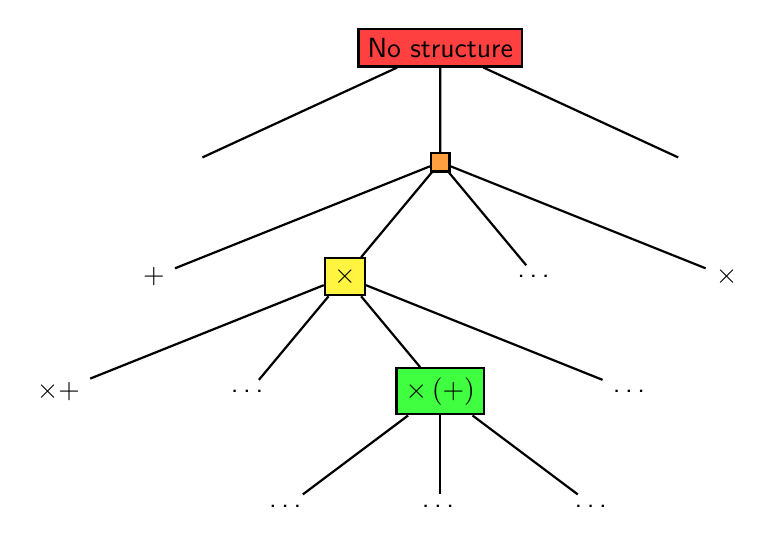
\begin{tikzpicture}
[sibling distance=0.26\columnwidth,-,thick, level distance=0.12\columnwidth]
%\footnotesize
\node[shape=rectangle,draw,thick,fill=red!75] {No structure}
  child {node {$\SE$}
  }
  child {node[shape=rectangle,draw,thick,fill=orange!75] {$\Lin$}
    [sibling distance=0.20\columnwidth]
    child {node {$\Lin + \Per$}}
    child {node[shape=rectangle,draw,thick,fill=yellow!75] {$\Lin \times \SE$}
      [sibling distance=0.20\columnwidth]
      child {node {$\Lin \times \SE + \SE$}}
      child {node {\ldots}}
      child {node[shape=rectangle,draw,thick,fill=green!75] {$\Lin \times \left( \SE + \Per \right)$}
        [sibling distance=0.16\columnwidth]
        child {node {\ldots}}
        child {node {\ldots}}
        child {node {\ldots}}
      }
      child {node {\ldots}}
    }
    %child {node {$\RQ \times \SE$}}
    child {node {\ldots}}
    child {node {$\Lin \times \Per$}}
  }
  child {node {$\Per$}};
\end{tikzpicture}


\end{center}

\newpage 

\mysection{Automatically describing model properties}

%\subsection*{How to automatically describe arbitrarily complex kernels:}
%\begin{itemize}
%\item The kernel is distributed into a sum of products
%\item Sums of kernels are sums of functions so each product is described separately
%\item Each kernel in a product modifies the model in a consistent way\ldots
%\item \ldots so one kernel is described by a noun phrase, and the others modify it
%\item Text descriptions are complemented by plots of the posterior
%\end{itemize}
%It is hard to write a lookup table to handle every kernel that the open-ended search might produce.  How to automate this?

%For a given dataset, the GPSS method produces a compound kernel composed of sums and products of the 6 base kernels.
%In this section, we describe how the properties of kernel functions reduce the task of natural-language summarization into relatively simple subproblems.

%\subsection{Summary}  
%\vspace{-0.08in}
%We have broken down the problem of describing arbitary compositions of kernels into two manageable parts.  First, we distribute the composite kernel into a sum of products.  Second, for each product of kernels, we describe the properties of products of kernels $\kSE$, $\kPer$, $\kC$ and $\kWN$, and then append descriptions of the properties of the modulating functions implied by products of $\kLin$ and $\kCP$.

\subsection*{Kernels can be distributed into a sum of products}

 
%For example:
\begin{equation*}
%\kSE \times \big( \kLin + \kLin \times ( \kPer + \kSE ) \big)
\kSE \times \big( \kLin + \kPer + \kSE \big)
\end{equation*}
\begin{centering}
becomes (after simplification)
\end{centering}
\begin{equation*}
%(\kSE \times \kLin) + (\kSE \times \kLin \times \kPer) + (\kSE \times \kLin).
(\kSE \times \kLin) + (\kSE \times \kPer) + (\kSE).
\end{equation*}


\subsection*{Sums of kernels correspond to sums of functions}




%
\definecolor{verylightblue}{rgb}{0.97,0.97,1}
\setlength{\fboxsep}{0pt}

\newcommand{\ltrim}{ 2 }
\newcommand{\rictrim}{ 2 }
%\newcommand{\airlinefig}[1]{\includegraphics[trim=20 0 12 20, clip, width=0.207\textwidth]{figures/#1}}
\newcommand{\airlinefigtwo}[1]{\includegraphics[trim=30 0 62 25, clip, width=0.18\columnwidth]{../figures/03-mauna2003_#1}}
\newcommand{\olduptext}[1]{\hspace{-1cm} \raisebox{ 0.8cm}{ {#1}} \hspace{-0.75cm} }
\newcommand{\uptext}[1]{ \raisebox{1.5cm}{ #1} }
%
\begin{tabular}{cc}
%\airlinefig{01-airline-months_all}&\hspace{0.6cm}\olduptext{$=$} \hspace{-0.1cm}
%\airlinefig{01-airline-months_1} & \olduptext{$+$}
%\airlinefig{01-airline-months_2} & \olduptext{$+$}
%\airlinefig{/01-airline-months_3} \\
\hspace{-3.5mm}
%\fbox{
\fcolorbox{blue}{white}{
\hspace{-3.5mm}
\begin{tabular}{c}
%\\[-0.7em]
\airlinefigtwo{all} \hspace{-3mm} \\
 entire signal
\end{tabular}
}
\begin{tabular}{cccccc}
\\%[1cm]
\uptext{$=$} & \airlinefigtwo{1} & \uptext{$+$} & \airlinefigtwo{2} & \uptext{$+$} & \airlinefigtwo{3} \\
& $\kSE \times \kLin$ & & $\kSE \times \kPer$ & & $\kSE$ \\
& smooth trend & + & periodicity & + & short-term deviation
\end{tabular}
\end{tabular}


\vspace{1.5\baselineskip}

If $f_1(x) \dist \gp{}(0, \kernel_1)$ and $f_2(x) \dist \gp{}(0, \kernel_2)$ then $f_1(x) + f_2(x) \dist \gp{}(0, \kernel_1 + \kernel_2)$.
Therefore, a sum of kernels can be described as a sum of functions.
%
%Thus, we can always exactly describe our model as a sum of these components, each of which is a product of base kernels.  The only remaining task is to produce a procedure for describing products of base kernels.





\subsection*{The compositional structure of products of kernels maps onto compositionally constructed sentences}

\vspace{1\baselineskip}

\centering
\begin{tabular}{l|l|l}
  Kernel & Noun phrase & Postmodifier phrase \\
  \midrule
  $\kWN$  & uncorrelated noise & n/a\\
  $\kC$   & constant & n/a \\
  $\kSE$  & smooth function & whose shape changes smoothly\\
  $\kPer$ & periodic function & modulated by a periodic function\\
  $\kLin$ & linear function & with linearly varying amplitude\\ 
  $\prod_k \kLin^{(k)}$ & polynomial & with polynomially varying amplitude\\
  $\prod_k \boldsymbol{\sigma}^{(k)}$ & n/a & which applies until / from [changepoint]
\end{tabular}

\vspace{1\baselineskip}

\raggedright
\subsection*{Example description}

{\large
\begin{align*}
  \underbrace{\kPer}_{\textnormal{\large periodic function}} \times 
  \underbrace{\kLin}_{\textnormal{\large with linearly growing amplitude}} \times 
  \underbrace{\boldsymbol{\sigma}}_{\textnormal{\large which applies until [date]}}
\end{align*}
}

$\kPer$ has been chosen to act as the noun while $\kLin$ and $\boldsymbol{\sigma}$ modify the description

%\centering
%\begin{tabular}{l|l}
%Product of Kernels & Description \\
%\midrule
%$\kPer$ & An exactly periodic function \\
%$\kPer \times \kSE$ & An approximately periodic function \\
%$\kPer \times \kSE \times \kLin$ & An approximately periodic function with linearly varying amplitude \\
%$\kLin$ & A linear function \\
%$\kLin \times \kLin$ & A quadratic function \\
%$\kPer \times \kLin \times \kLin$ & An exactly periodic function with quadratically varying amplitude\\
%\end{tabular}

\vspace{1\baselineskip}

\mysection{Visit the website - try the (simple) demo}

\centering
\def\UrlFont{\bfseries}
\huge \url{www.automaticstatistician.com}

\end{multicols}

\end{poster}

\end{document}

